\documentclass[a4paper,12pt,titlepage]{article}

\usepackage[german,ngerman]{babel}
\usepackage{fontspec}
\setmainfont{Calibri}
\usepackage{graphicx}
\usepackage{hyperref}
\usepackage{caption}

\begin{document}

\begin{titlepage}
    \centering
    \vspace*{2cm}
    {\LARGE\bfseries Automaten und formale Sprachen Blatt 2\par}
    \vspace{2cm}
    {\Large Jan Lucca Agricola (275867) \& Jakob Schulz (275258)\par}
    \vspace{2cm}
    {\large\today\par}
\end{titlepage}

\section{Aufgabe}
\begin{enumerate}
\item $L(r\ |\ r^*) = \{\epsilon, r, rr, rrr,...\}$
\item $L((r \cdot t)^*) = \{\epsilon, rt, rtrt, rtrtrt,...\}$
\item $L(r^* \cdot t^*) = \{\epsilon, r, t, rt, rr, tt, rrt, rtt, rrr,...\}$
\item $L((t \cdot r)^*) = \{\epsilon, tr, trtr, trtrtr,...\}$
\item $L((r\ |\ t)^*) = \{\epsilon, r, t, rr, tt, rt, tr, rtrt, rttr, trrt, rrr, ttt,...\}$
\item $L(r^*\ |\ t^*) = \{\epsilon, r, t, rr, tt, rrr, ttt,...\}$
\item $L((0^*\ \cdot\  1)^*\ \cdot\ 0^*) = \{\epsilon, 0, 1, 10, 01, 010, 101, 1011, 0101, 01010, 001, 110, 0010, 0100, 00100, ...\}$
\item $L((1\ |\ 0)^*) = \{\epsilon, 1, 0, 11, 00, 10, 01, 010, 100, 101, 111, 000, 11001,...\}$
\end{enumerate}
\section{Aufgabe}
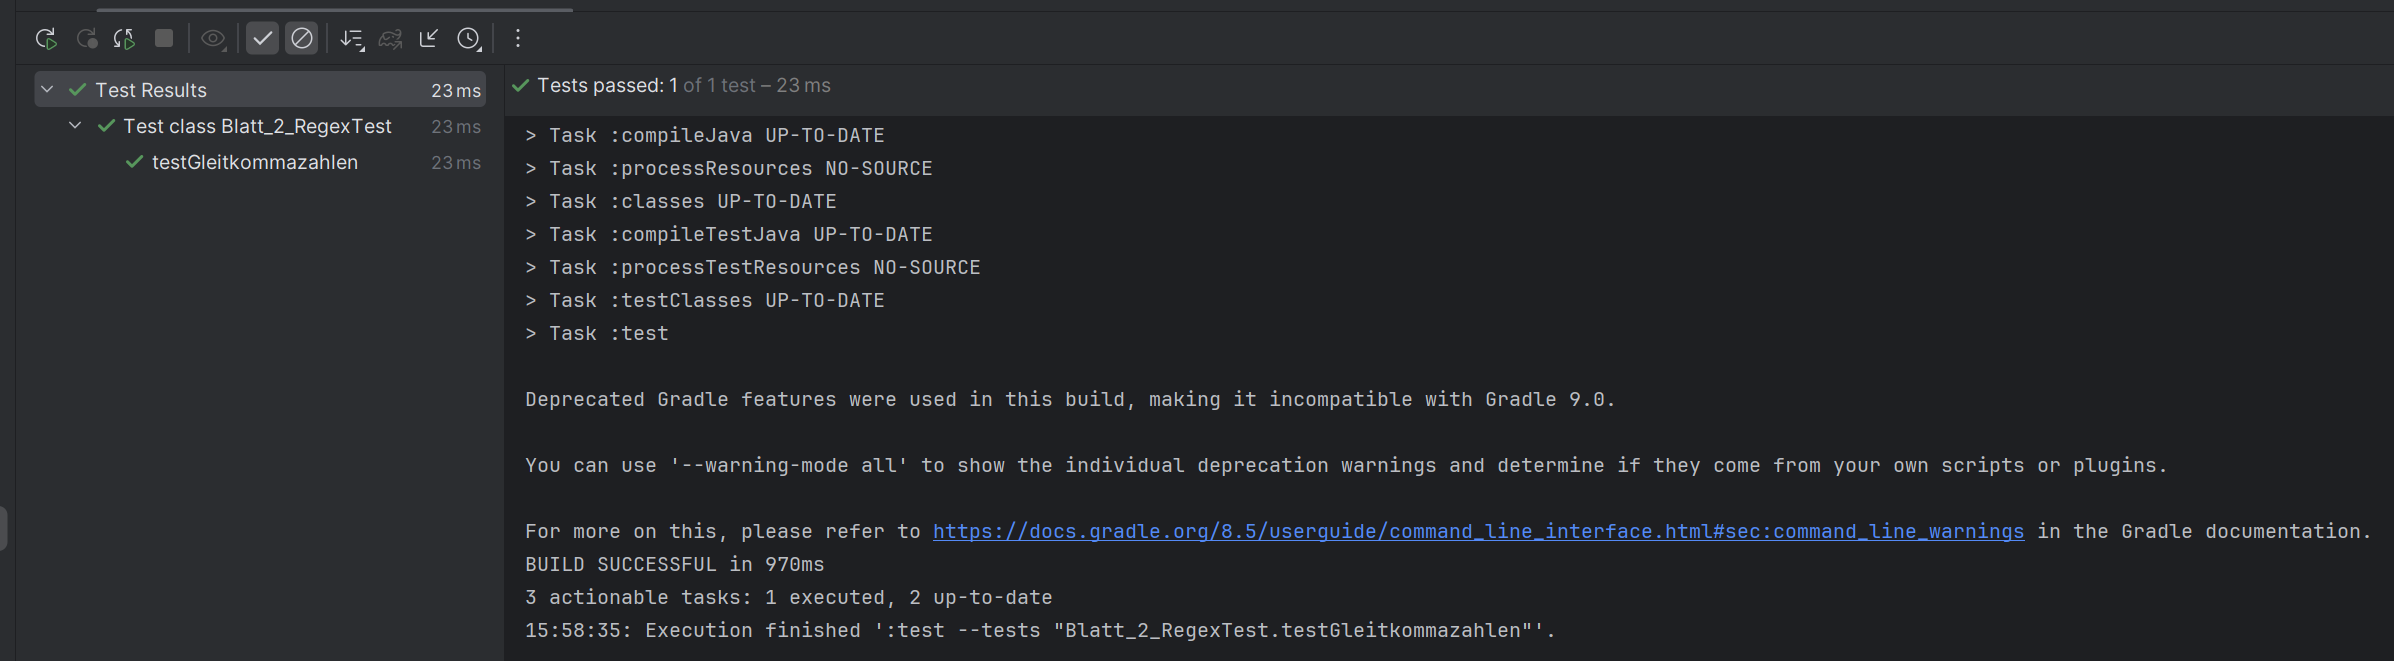
\includegraphics[width=0.9\textwidth]{testGleitkommazahlen.png}\\
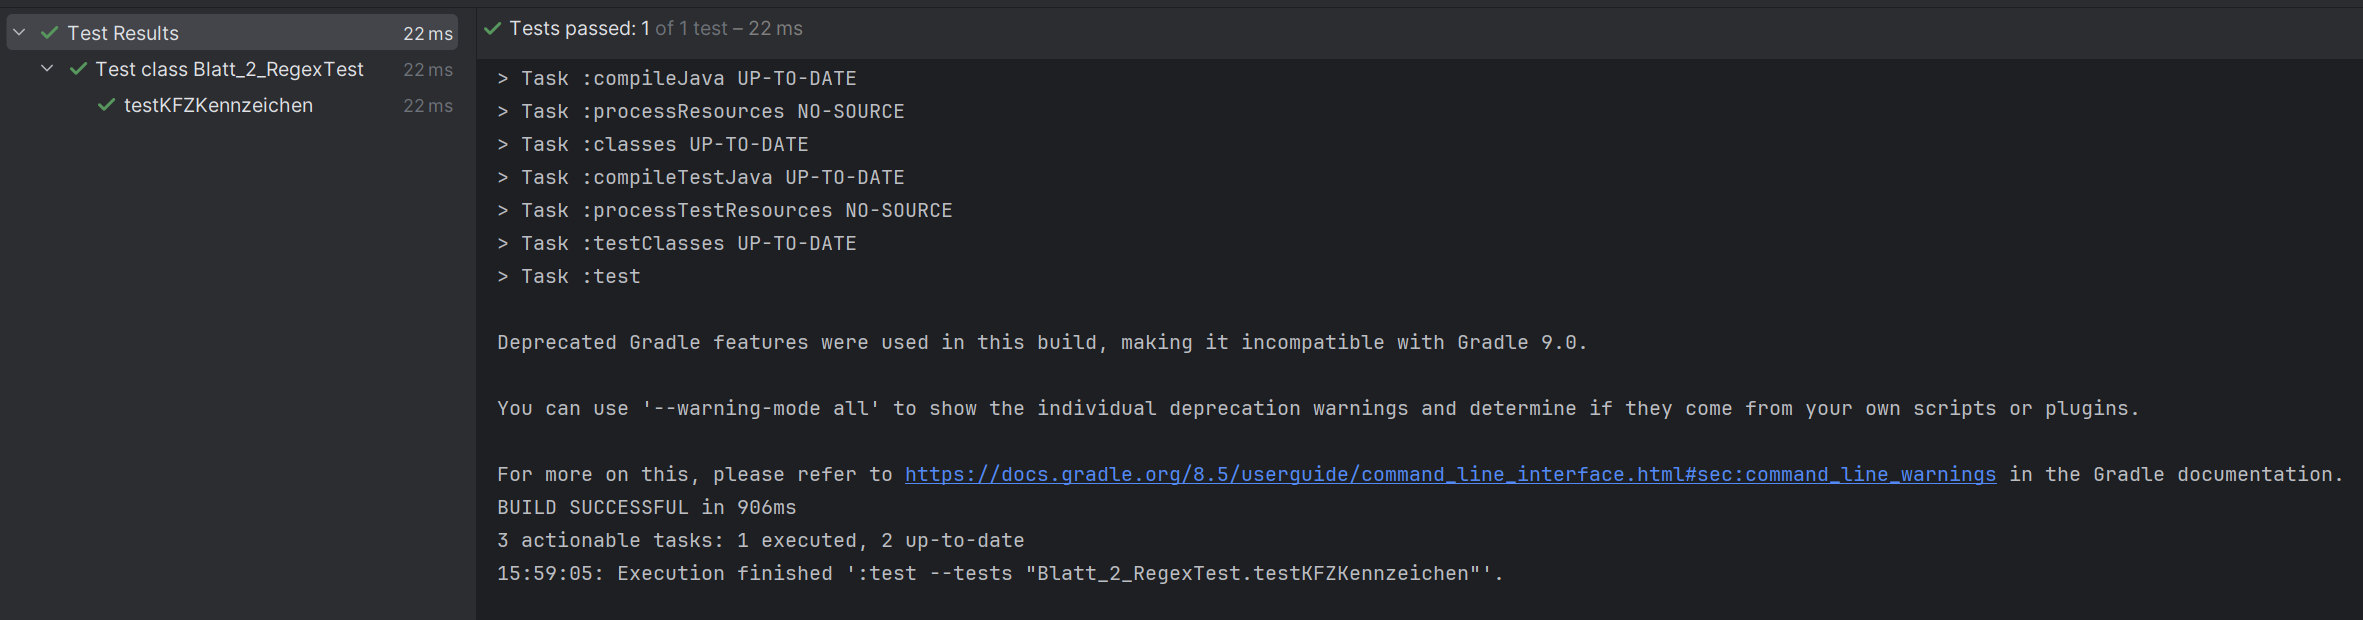
\includegraphics[width=0.9\textwidth]{testKFZKennzeichen.png}\\
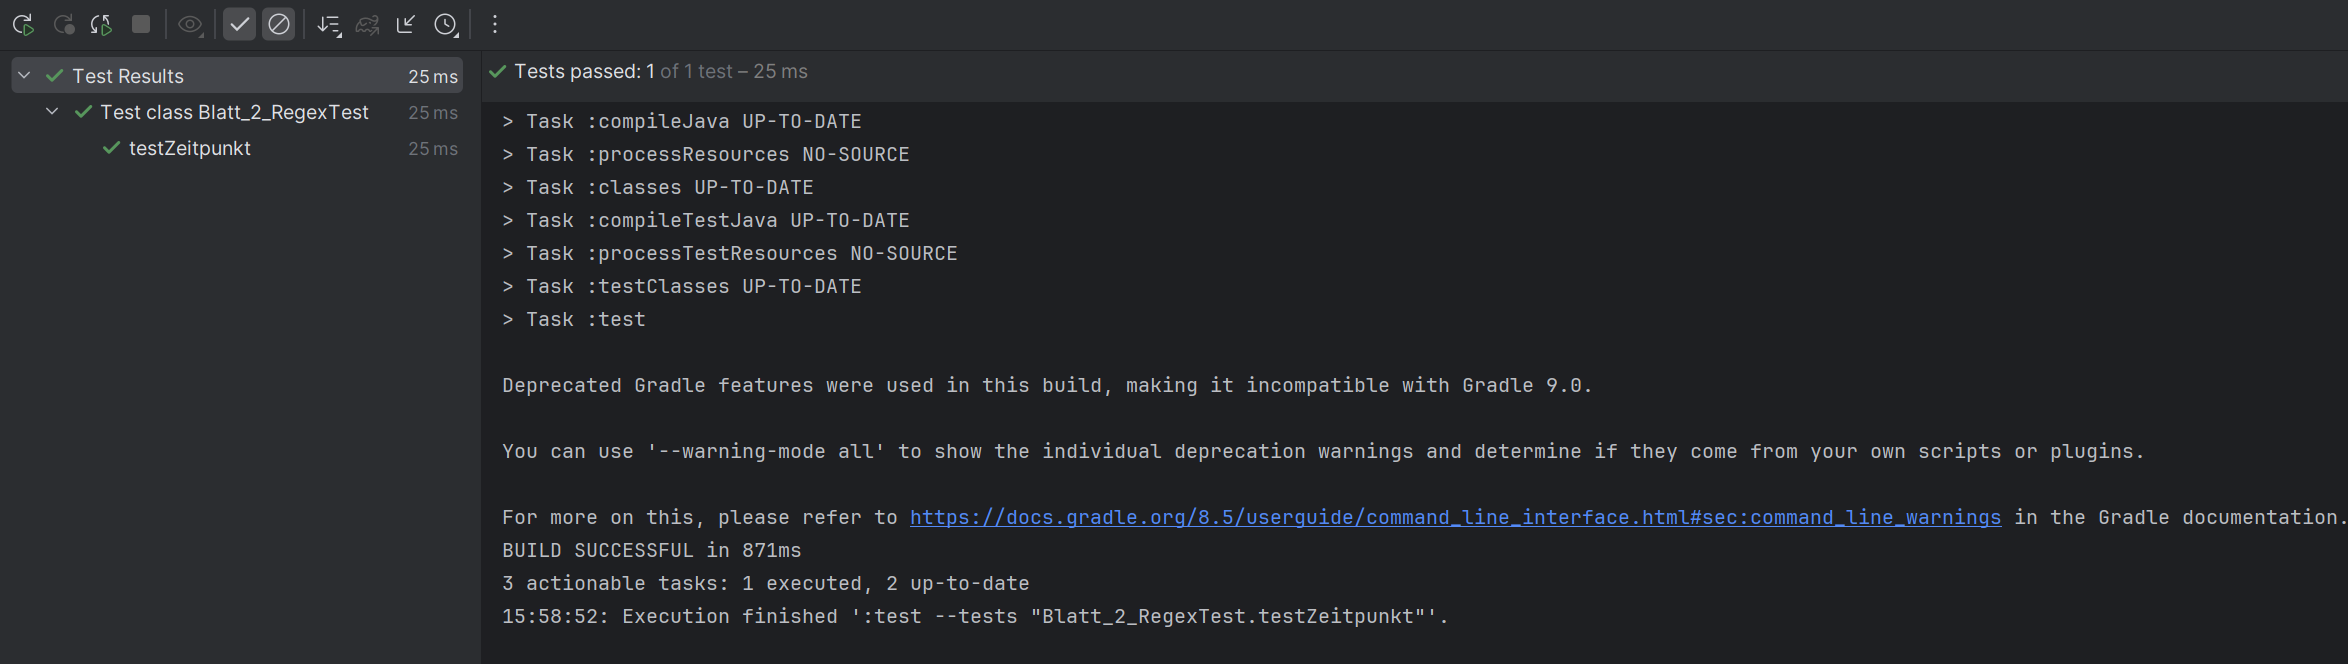
\includegraphics[width=0.9\textwidth]{testZeitpunkt.png}\\
\end{document}
